\documentclass[14pt,a4paper]{scrartcl}
\usepackage[left=1.5cm,right=1.5cm,
    top=1.5cm,bottom=1.5cm,bindingoffset=0cm]{geometry}

\usepackage[T1,T2A]{fontenc}
\usepackage[utf8]{inputenc}
\usepackage[english,russian,ukrainian]{babel}
\usepackage{tabularx}
\usepackage{amssymb}
\usepackage{color}
\usepackage{amsmath}
\usepackage{mathrsfs}
\usepackage{listings}
\usepackage{graphicx}
\graphicspath{ {./images/} }
%\usepackage{draftwatermark} не будет лезть на картинки
\usepackage[printwatermark]{xwatermark}%будет лезть на картинки
\usepackage{lipsum}
\usepackage{xcolor}
\usepackage{tikz}
\definecolor{lgreen}{rgb}{0.5,1,1}
\definecolor{n}{rgb}{1,0.5,0.5}
\definecolor{n1}{rgb}{1,1,0.5}
\definecolor{n3}{rgb}{1,0.7,0.9}
 \usepackage{csvsimple}
 \usepackage{supertabular}
\usepackage{pdflscape} 



\begin{document}
\pagestyle{plain}
\pagecolor{white}






\begin{titlepage}
  \begin{center}
    \large
    Національний технічний університет України \\ "Київський політехнічний інститут імені Ігоря Сікорського"
     
       
    Факультет Електроніки
     
    Кафедра мікроелектроніки
    \vfill
      
    \textsc{ЗВІТ}\\
     
    {\Large Про виконання розрахункової роботи №1\\
      з дисципліни: «Теорія поля»\\[1cm]
      
   % ДОСЛІДЖЕННЯ ВИПРЯМЛЯЮЧИХ НАПІВПРОВІДНИКОВИХ ДІОДІВ\\
    
    }
  \bigskip
\end{center}
\vfill
 
\newlength{\ML}
\settowidth{\ML}{«\underline{\hspace{0.4cm}}» \underline{\hspace{2cm}}}
\hfill
\begin{minipage}{1\textwidth}
Виконавець:\\
Студент 3-го курсу \hspace{4cm} $\underset{\text{(підпис)}}{\underline{\hspace{0.2\textwidth}}}$  \hspace{1cm}А.\,С.~Мнацаканов\\
\vspace{1cm}

Превірила: \hspace{6.1cm} $\underset{\text{(підпис)}}{\underline{\hspace{0.2\textwidth}}}$  \hspace{1cm}Т.\,А.~Саурова\\

\end{minipage}

\vfill

\begin{center}
2020
\end{center}
\end{titlepage}


 

\begin{center}
\textbf{ЗАВДАННЯ} \\
\end{center}

\textbf{1.} Розрахувати розподіл потенціалу в міжелектродному просторі польового транзистора (варіант конструкції вибирається за передостанньою цифрою номера залікової книжки) з точністю до 0,01 В. Номер варіанту обирається за останньою цифрою номера залікової книжки.\par

\textbf{2.} Побудувати картини поля за допомогою еквіпотенціалей і векторів напруженості електричного поля. Побудувати косокутну проекцію потенціального рельєфу U(x,y) = $-e\cdot V(x,y)$\\
\begin{figure}[h]
\center{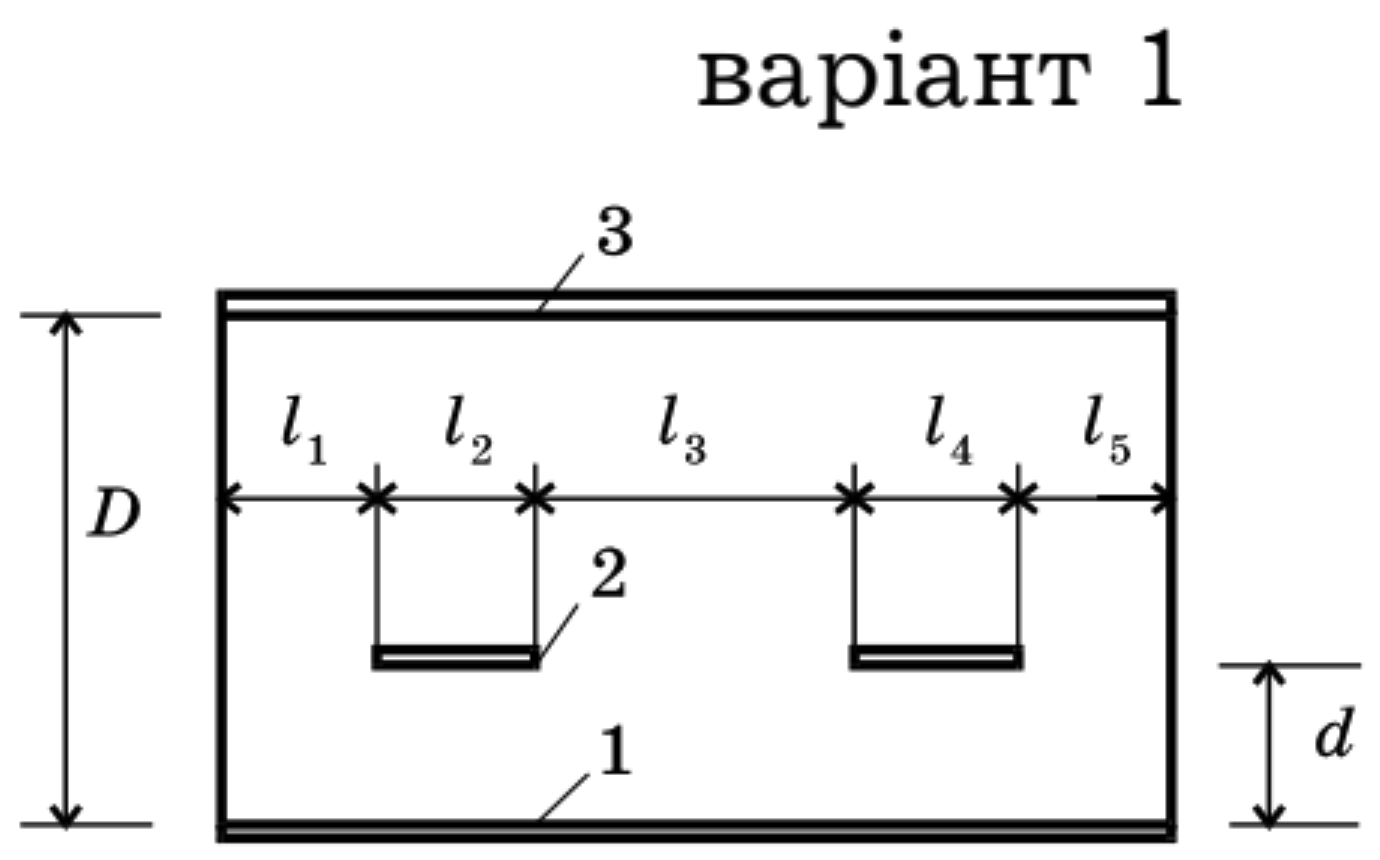
\includegraphics[width=0.5\linewidth]{var1.png} \\
$ l_1 = l2 = l_3/2 = l_4 = l_5 = 1,0$ мкм, d = 1,0 мкм,\\ D = 3,0 мкм 1 – витік, 2 – затвор, 3 – стік }
\end{figure}

\begin{center}
\vspace{0.1cm}
\begin{Large}
\begin{tabular}{ | c |  c |  c |  c |}
\hline
вар. № & 4   \\ 
\hline
$-V_{3B},B$ & 0.5   \\ 
\hline
$V_{CB}, B$ & 3   \\ 
\hline
\end{tabular}
\end{Large}
\vspace{0.2cm}
\end{center}

\newpage
\begin{center}
\textbf{РОЗРАХУНКИ} \\
\end{center}


\begin{center}
\begin{figure}[h]
\center{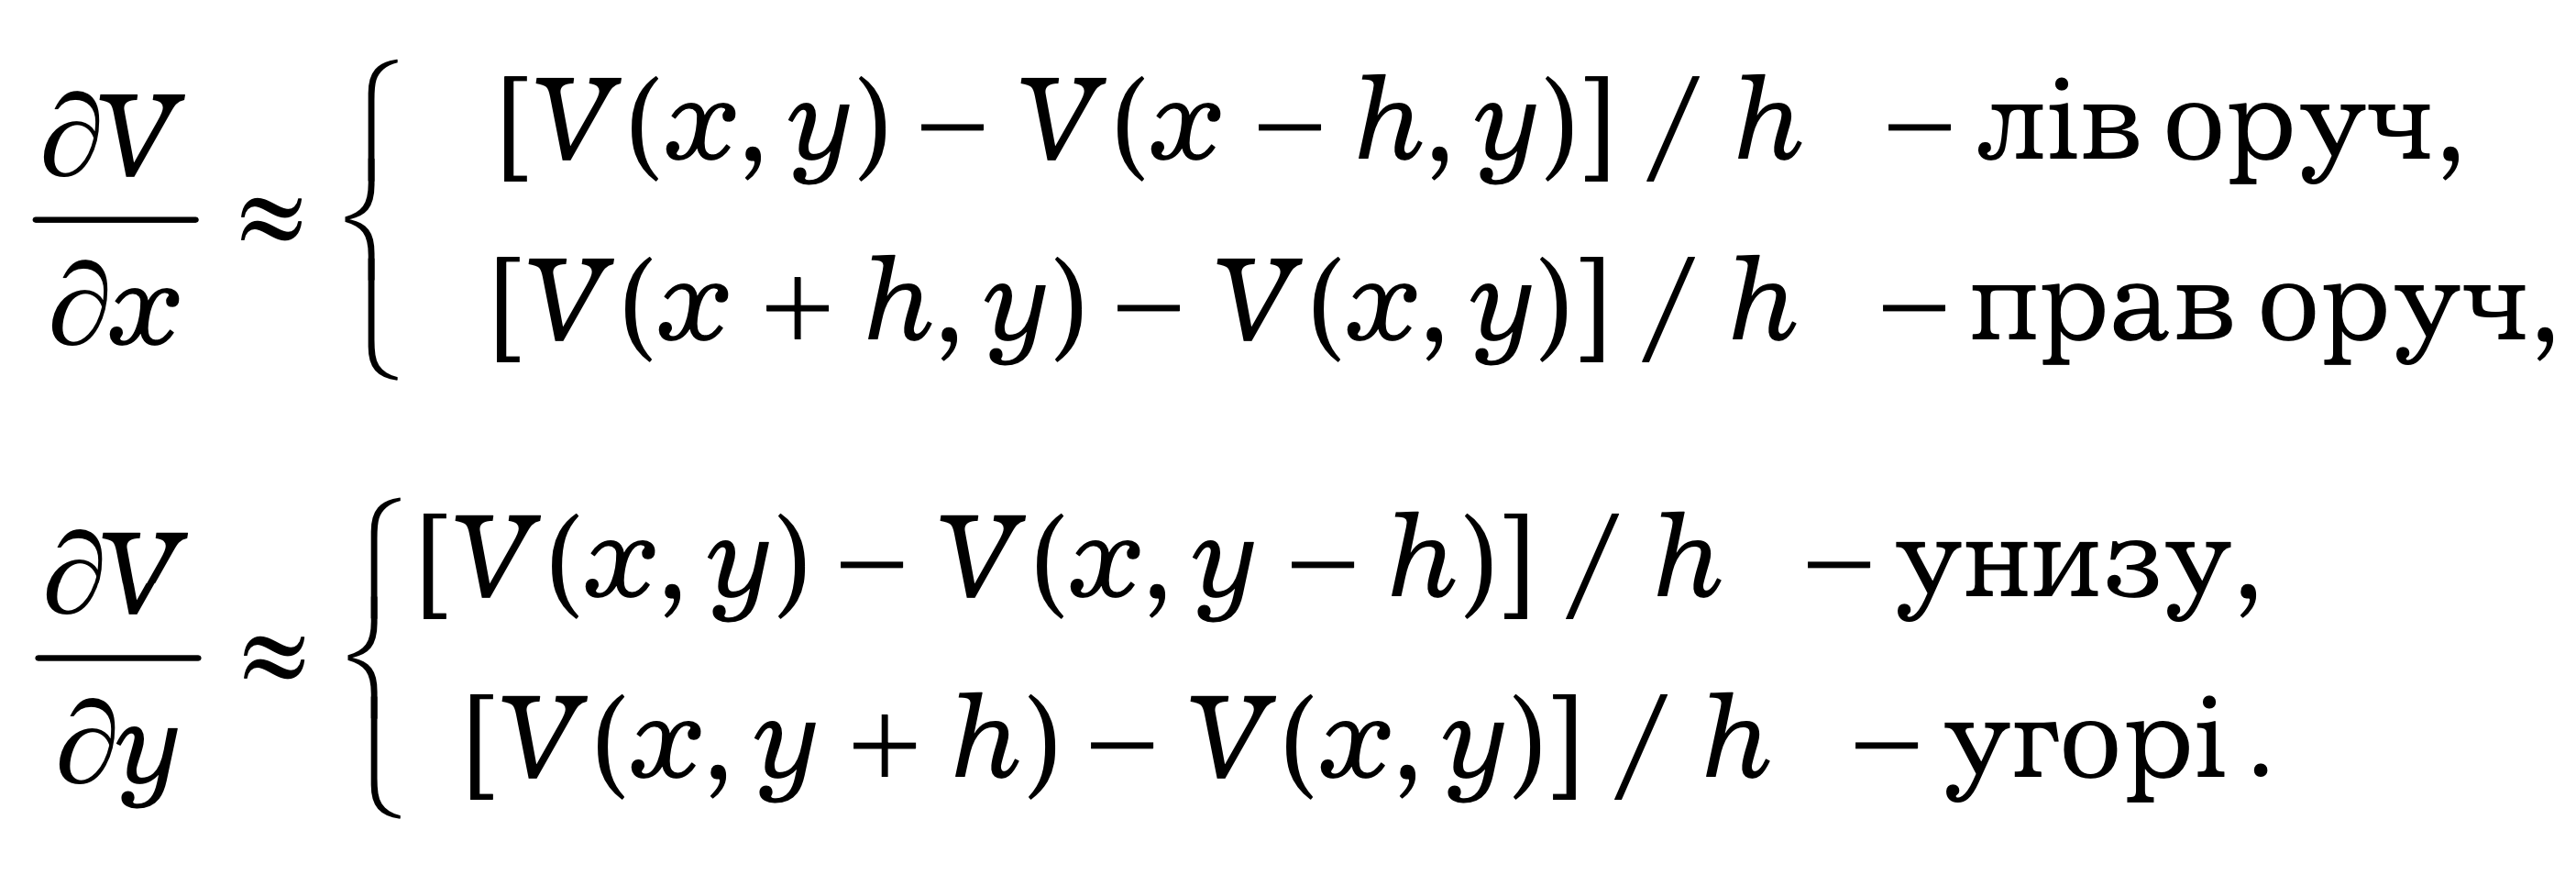
\includegraphics[height=4cm, width=12cm]{f.png}}
\end{figure}
\end{center}

\begin{center}
\begin{figure}[h]
\center{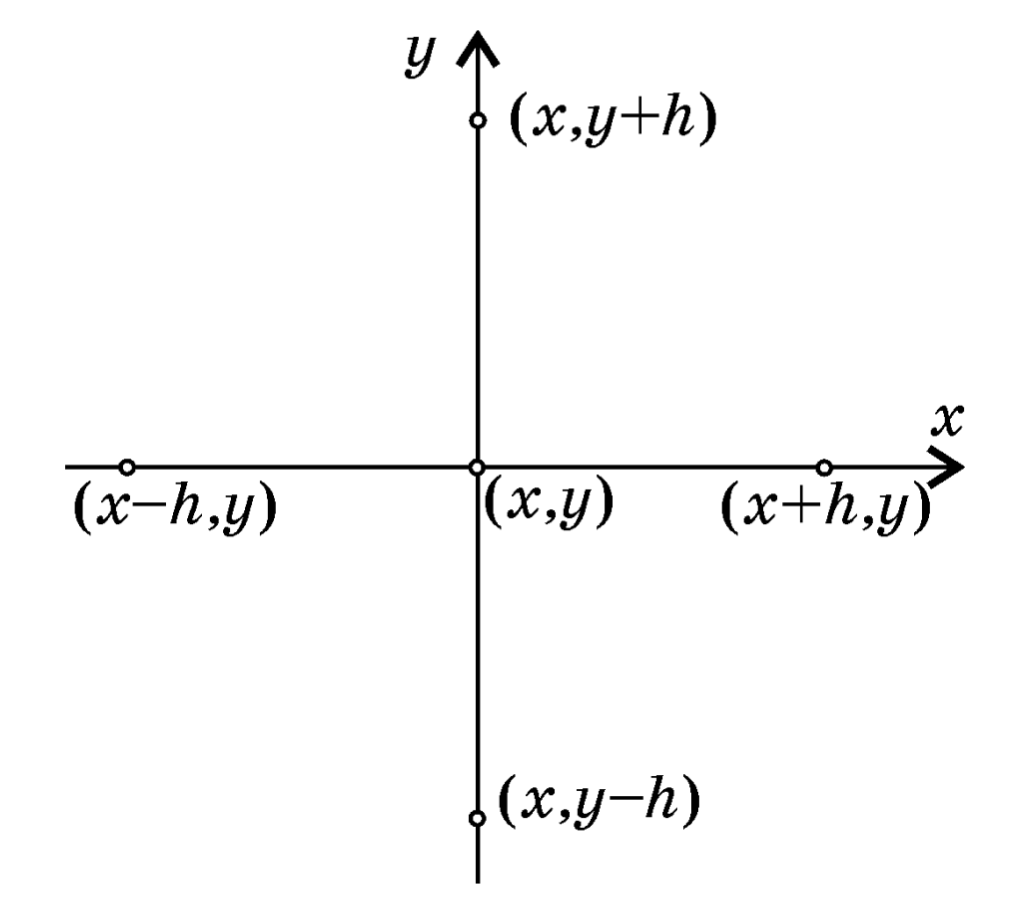
\includegraphics[height=8cm, width=8cm]{5t.png}}
\caption{П'ятиточкова схема для обчислення похідних через кінцеві прирости і розрахунку потенціалів..}
\label{ris:image5}
\end{figure}
\end{center}

\newpage
Представимо всю площину транзистора як  дискретний масив точок розмірністю 25х13. 

\begin{center}
\begin{figure}[h]
\center{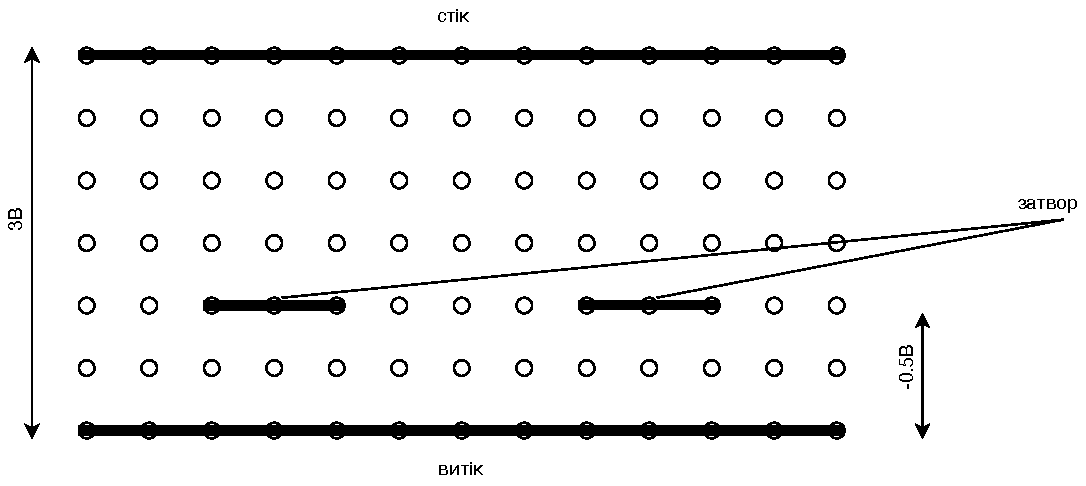
\includegraphics[width=1\linewidth]{0.pdf}}
\caption[wec]{Дисткретизація простору інтегрування за допомогою сітки з постійним кроком 0.5 мкм\footnotemark}
\label{ris:image}
\end{figure}
\footnotetext{Зауважимо, що для подальших розрахунків крок було зменшено вдвічі, тобто 0.25 мкм.}
\end{center}


При цьому двомірне рівняння Лапласа
\begin{equation}
\dfrac{\partial^2 V}{\partial x^2} +\dfrac{\partial^2 V}{\partial y^2} =0
\label{eq:ref}
\end{equation}
наближено заміняється наступним алгебраічним рівнянням:
\begin{equation}
V ( x + h, y ) + V ( x-h, y ) + V ( x, y + h ) + V ( x, y-h ) - 4 V ( x, y ) = 0
\label{eq:ref}
\end{equation}








\newpage

Розрахунок напруженості електричного поля провадиться за співвідношення $E_x$=$-\dfrac{\partial V}{\partial x}$, $E_y$=$\dfrac{\partial V}{\partial y}$що наближено обчислюються через кінцеві різниці. Використовуючи значення похідних зліва і справа, можна знайти середнє арифметичне
\begin{equation}
E_{x\text{ }i,j} = \dfrac{V_{(i-1),j}  + V_{(i+1),j}}{2}
\label{eq:ref}
\end{equation}
\begin{equation}
E_{y\text{ }i,j} = \dfrac{V_{i,(j-1)}  + V_{i,(j+1)}}{2}
\label{eq:ref}
\end{equation}








 


Наступним кроком я графічно зобразив веркори напруженості електричного поля в нашому польовому транзисторі (рис. \ref{ris:image3}). Дивлячись на цей рисунок можна чітко побачити що електричне поле яке прямує із стоку до затвору набагато сильніше ніж те що йде йому на зустріч, про що свідчать довжини стрілок.\\

\begin{center}
\begin{figure}[h]
\center{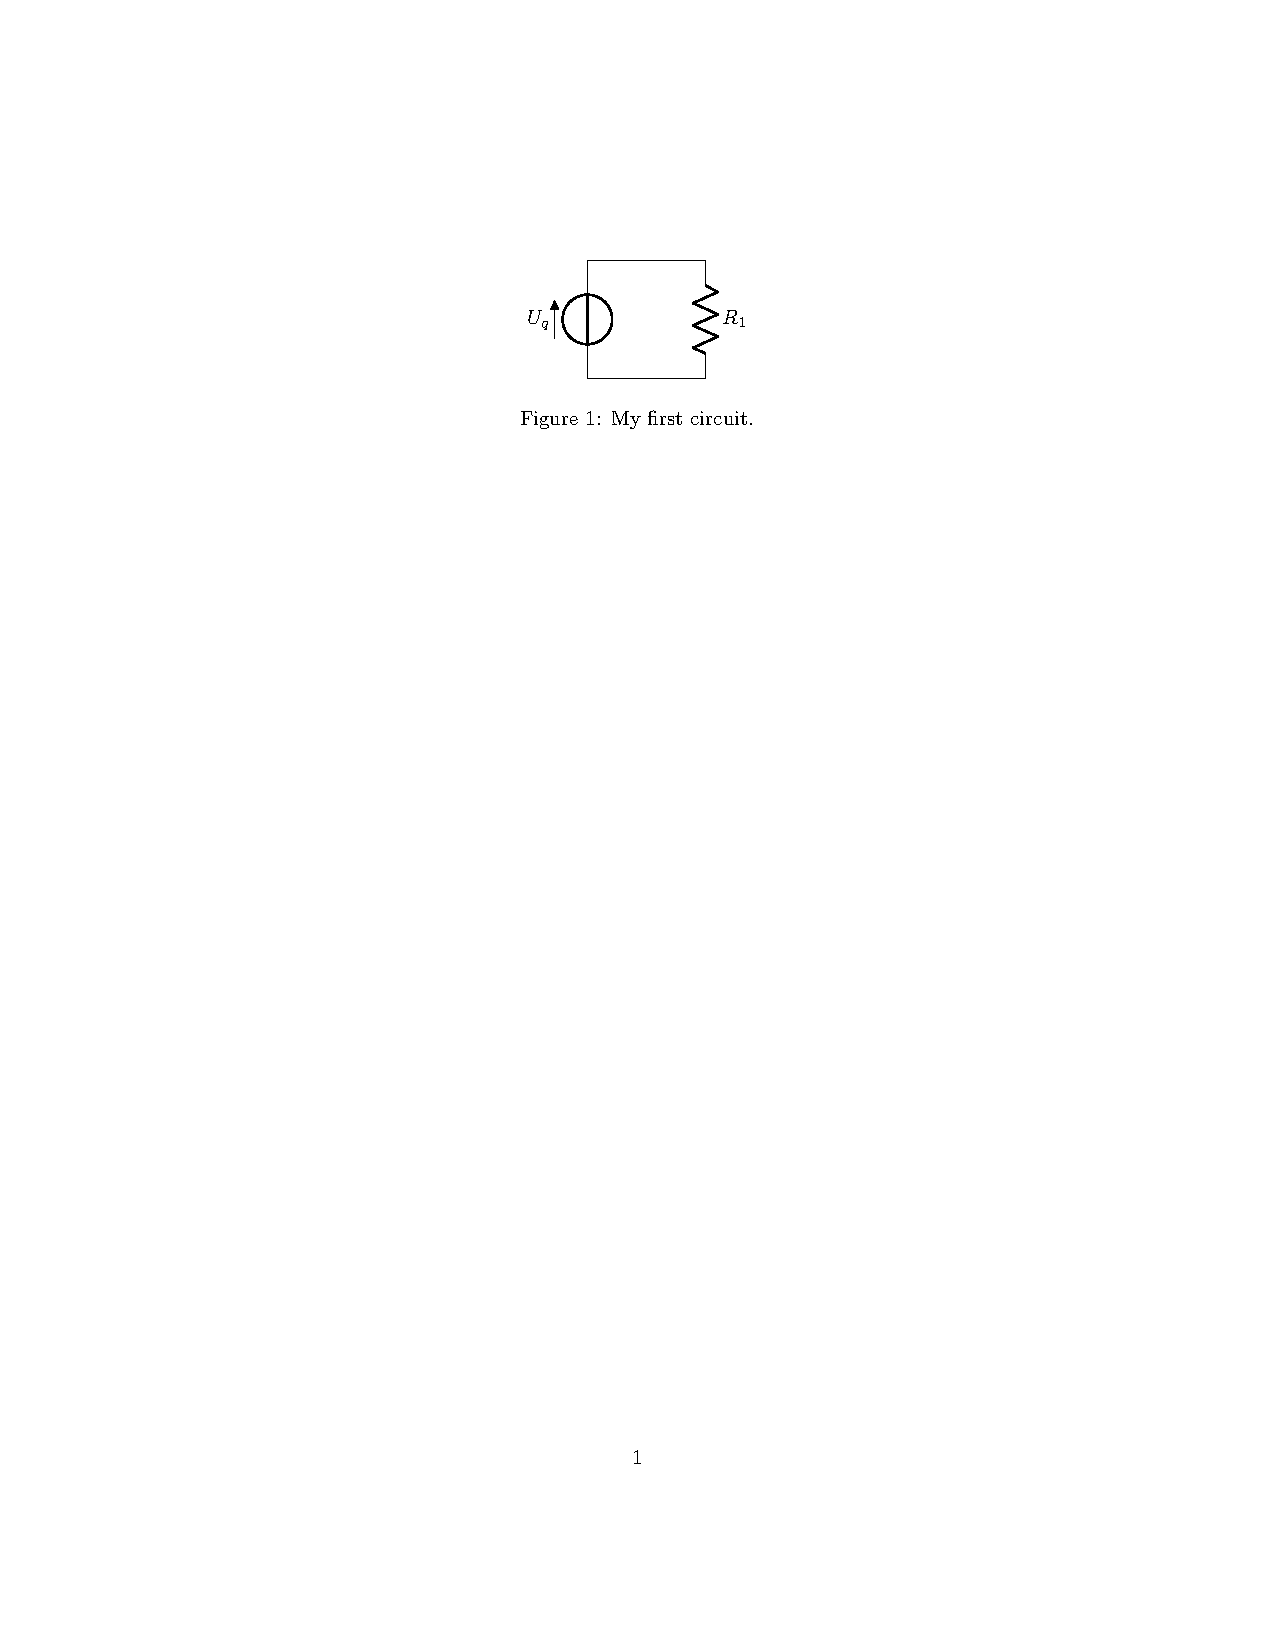
\includegraphics[width=1\linewidth]{1.pdf}}
\caption{Картина поля за допомогою векторів напруженості електричного поля.}
\label{ris:image3}
\end{figure}

\newpage

\begin{figure}[h]

\caption{Косокутна проекція потенціального рельєфу U(x,y) = -eV(x,y).}
\label{ris:image4}
\end{figure}
\end{center}







\clearpage
Висновок: \\








\clearpage
\begin{center}
\textbf{ДОДАТОК}
\end{center}















\end{document}